% Part 1 report: why these KEMs, what a KEM is, DH -> KEM, and the E1 (performance)
% and E4 (correctness) results on Apple M4 and Intel i7-1185G7.
% Build: python3 analysis/part1_figures.py && cd report/part1 && latexmk -pdf part1.tex
\documentclass[10.5pt,a4paper]{article}
\usepackage[a4paper,margin=2.1cm,top=2.2cm,bottom=2.3cm]{geometry}
\usepackage[T1]{fontenc}
\usepackage[utf8]{inputenc}
\usepackage{charter}
\usepackage[scaled=0.9]{helvet}
\usepackage{amsmath,amssymb}
\usepackage{microtype}
\usepackage{graphicx}
\usepackage{booktabs,tabularx,multirow,array}
\usepackage{xcolor}
\usepackage{tikz}
\usetikzlibrary{arrows.meta,positioning,calc,fit,backgrounds,shapes.geometric}
\usepackage[most]{tcolorbox}
\usepackage{enumitem}
\usepackage{caption}
\usepackage{float}
\usepackage[hidelinks]{hyperref}
\usepackage{fancyhdr}

\DeclareUnicodeCharacter{00B5}{\ensuremath{\mu}}
\DeclareUnicodeCharacter{00D7}{\ensuremath{\times}}
\DeclareUnicodeCharacter{2192}{\ensuremath{\rightarrow}}

\definecolor{mfour}{HTML}{2A78D6}
\definecolor{iseven}{HTML}{EB6834}
\definecolor{refc}{HTML}{1BAF7A}
\definecolor{optc}{HTML}{6250D6}
\definecolor{osslc}{HTML}{E87BA4}
\definecolor{fmlkem}{HTML}{1BAF7A}
\definecolor{fhqc}{HTML}{EDA100}
\definecolor{ffrodo}{HTML}{E87BA4}
\definecolor{fmce}{HTML}{008300}
\definecolor{ink}{HTML}{0B0B0B}
\definecolor{ink2}{HTML}{52514E}
\definecolor{muted}{HTML}{898781}
\definecolor{gridc}{HTML}{E1E0D9}
\definecolor{wash}{HTML}{F4F3EF}
\definecolor{good}{HTML}{006300}

\setlist{itemsep=1pt,topsep=3pt,parsep=0pt,leftmargin=1.2em}
\captionsetup{font=small,labelfont=bf,labelsep=period,skip=4pt}
\setlength{\parindent}{0pt}
\setlength{\parskip}{4pt}
\renewcommand{\arraystretch}{1.12}
\pagestyle{fancy}
\fancyhf{}
\fancyhead[L]{\small\sffamily\color{ink2}Post-quantum KEMs · Part 1: performance (E1) and correctness (E4)}
\fancyhead[R]{\small\sffamily\color{ink2}\thepage}
\renewcommand{\headrulewidth}{0.3pt}

\newcommand{\sect}[1]{\section{#1}}
\newcommand{\key}[1]{\textbf{#1}}
\newtcolorbox{takeaway}[1][Takeaways]{colback=wash,colframe=wash,boxrule=0pt,arc=2pt,left=7pt,right=7pt,
  top=5pt,bottom=5pt,fonttitle=\sffamily\bfseries\small,coltitle=ink,title={#1},attach title to upper={\par}}
\newtcolorbox{defbox}[1]{colback=white,colframe=mfour!60,boxrule=0.6pt,arc=2pt,left=7pt,right=7pt,top=5pt,
  bottom=5pt,fonttitle=\sffamily\bfseries\small,coltitle=white,colbacktitle=mfour,title={#1}}

\newcommand{\fxMecdh}{62.5\,µs}
\newcommand{\relMecdh}{1}
\newcommand{\fxMmlkemI}{17.6\,µs}
\newcommand{\relMmlkemI}{0.28}
\newcommand{\invMmlkemI}{3.6}
\newcommand{\fxMmlkemIII}{28\,µs}
\newcommand{\relMmlkemIII}{0.45}
\newcommand{\invMmlkemIII}{2.2}
\newcommand{\fxMmlkemV}{42.4\,µs}
\newcommand{\relMmlkemV}{0.68}
\newcommand{\invMmlkemV}{1.5}
\newcommand{\fxMhybrid}{100\,µs}
\newcommand{\relMhybrid}{1.6}
\newcommand{\fxMhqcI}{3.41\,ms}
\newcommand{\relMhqcI}{55}
\newcommand{\fxMfrodoI}{2.72\,ms}
\newcommand{\relMfrodoI}{43}
\newcommand{\fxMmceI}{52.6\,ms}
\newcommand{\relMmceI}{841}
\newcommand{\fxIecdh}{115\,µs}
\newcommand{\relIecdh}{1}
\newcommand{\fxImlkemI}{20.8\,µs}
\newcommand{\relImlkemI}{0.18}
\newcommand{\invImlkemI}{5.5}
\newcommand{\fxImlkemIII}{33.2\,µs}
\newcommand{\relImlkemIII}{0.29}
\newcommand{\invImlkemIII}{3.5}
\newcommand{\fxImlkemV}{46.4\,µs}
\newcommand{\relImlkemV}{0.4}
\newcommand{\invImlkemV}{2.5}
\newcommand{\fxIhybrid}{191\,µs}
\newcommand{\relIhybrid}{1.7}
\newcommand{\fxIhqcI}{7.35\,ms}
\newcommand{\relIhqcI}{64}
\newcommand{\fxIfrodoI}{2.23\,ms}
\newcommand{\relIfrodoI}{19}
\newcommand{\fxImceI}{38.7\,ms}
\newcommand{\relImceI}{337}
\newcommand{\eFourVectors}{1,332}
\newcommand{\eFourChecks}{69}


\tikzset{
  party/.style={draw=ink2,rounded corners=2pt,minimum width=2.6cm,minimum height=0.8cm,font=\sffamily\small\bfseries,fill=wash},
  op/.style={draw=ink2!70,rounded corners=2pt,font=\sffamily\scriptsize,fill=white,align=center,inner sep=3pt},
  msg/.style={-{Stealth[length=2.2mm]},thick,ink2},
  lbl/.style={font=\sffamily\scriptsize,ink2,align=center},
}

\begin{document}

% ------------------------------------------------------------------ title
\begin{titlepage}
\sffamily
\vspace*{0.4cm}
{\color{ink2}\large Cybersecurity Lab 1 · ELTE Faculty of Informatics · Autumn 2026}\par
\vspace{0.6cm}
{\Huge\bfseries Comparative study of\\[2pt] post-quantum key-encapsulation\\[2pt] mechanisms\par}
\vspace{0.4cm}
{\LARGE\color{mfour} Part 1: performance (E1) and correctness (E4)\par}
\vspace{0.8cm}
{\large Hamdan Al-Jabri}\par
{\color{ink2} 11 October 2026}\par
\vspace{0.9cm}

{\bfseries\large At a glance}\par\smallskip
\newcommand{\tile}[3]{\begin{tcolorbox}[colback=wash,colframe=wash,arc=3pt,left=8pt,right=8pt,top=6pt,bottom=6pt]
{\fontsize{20}{22}\selectfont\bfseries #1}\par\vspace{2pt}{\small\bfseries #2}\par\vspace{1pt}{\footnotesize\color{ink2}#3}\end{tcolorbox}}
\begin{tcbraster}[raster columns=2,raster equal height,raster column skip=8pt,raster row skip=8pt]
\tile{\eFourChecks/\eFourChecks}{correctness checks pass on both machines}{KATs, NIST ACVP (FIPS 203), random round trips, ref$\leftrightarrow$opt, liboqs$\leftrightarrow$OpenSSL; \eFourVectors{} vectors each}
\tile{\invMmlkemIII× / \invImlkemIII×}{ML-KEM-768 is cheaper than X25519}{compute for a full key exchange vs classical X25519 ECDH (M4 / i7)}
\tile{\relMhybrid× / \relIhybrid×}{the deployed hybrid vs X25519}{X25519MLKEM768 costs exactly its two parts added together}
\tile{\relMfrodoI–\relMmceI×}{the conservative KEMs vs X25519}{HQC, FrodoKEM and Classic McEliece at level 1 (M4)}
\tile{25–16,000×}{more bytes on the wire than X25519}{ML-KEM-768: 2,272\,B vs 64\,B; Classic McEliece: up to 1\,MB public keys}
\tile{up to 1,400×}{speed-up from AVX2 code}{McEliece decaps on the i7; NEON exists only for ML-KEM, so the M4 gains 1.4–1.7× there}
\end{tcbraster}

\vfill
{\small\color{ink2}
Measurements: Apple M4 (ARM64, Docker Desktop) and Intel Core i7-1185G7 (x86-64, WSL2), liboqs 0.16.0 and
OpenSSL 3.5.8.\\ All figures and tables are generated by \texttt{analysis/part1\_figures.py} from \texttt{results/raw}.\\
Code and data: \texttt{github.com/hsh1994-ux/pq-kem-study}.\par}
\end{titlepage}

\tableofcontents
\vspace{0.6cm}

\begin{takeaway}[Scope of Part 1]
\begin{itemize}
\item \key{RQ1 (cost).} How much computation, memory and bandwidth does each KEM need, compared with classical X25519? Answered by \key{E1}.
\item \key{RQ4 (correctness).} Do the implementations we measure compute the right thing, on both architectures and across libraries? Answered by \key{E4}.
\item E2 (TLS handshakes) and E3 (timing side channels) are reported in Part 2.
\end{itemize}
\end{takeaway}

\newpage
% ------------------------------------------------------------------ 1
\sect{Why these four KEMs}

Post-quantum KEMs fall into a few families, depending on the hard problem their security rests on. We picked one representative from each corner of a $2\times2$ map: \key{lattice vs.\ code-based}, and \key{structured vs.\ unstructured} (Figure~\ref{fig:map}).

\begin{figure}[H]
\centering
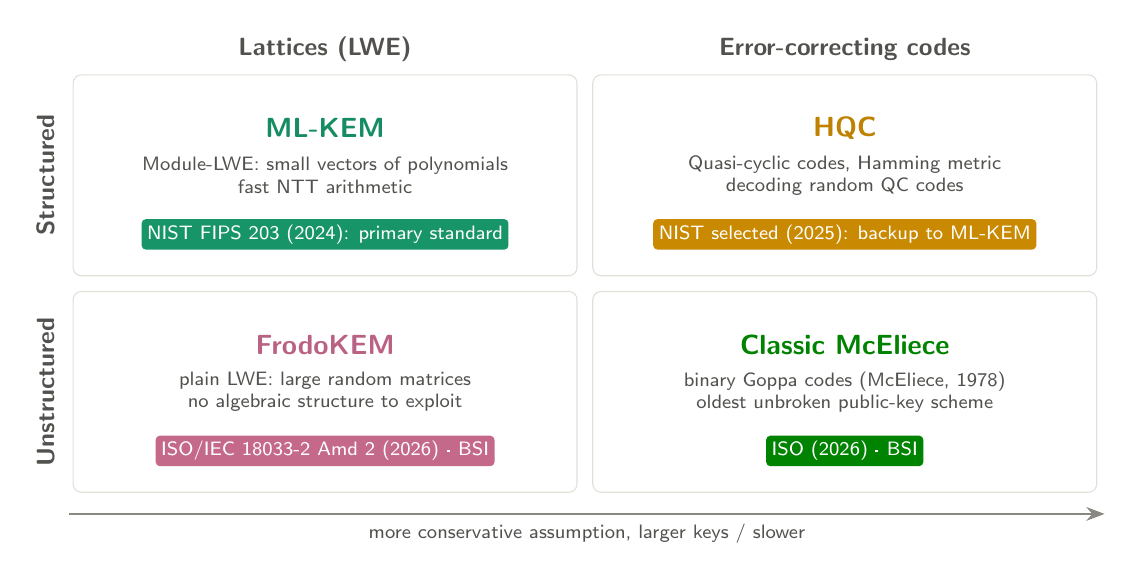
\begin{tikzpicture}[font=\sffamily\small,
  cell/.style={draw=gridc,fill=white,minimum width=6.4cm,minimum height=2.55cm,rounded corners=3pt,align=center},
  kem/.style={font=\sffamily\bfseries\normalsize},
  tag/.style={font=\sffamily\scriptsize,rounded corners=1.5pt,inner sep=2pt,text=white}]
\node[cell] (a) at (0,0) {};
\node[cell] (b) at (6.6,0) {};
\node[cell] (c) at (0,-2.75) {};
\node[cell] (d) at (6.6,-2.75) {};
% labels
\node[font=\sffamily\bfseries\small,ink2] at (0,1.6) {Lattices (LWE)};
\node[font=\sffamily\bfseries\small,ink2] at (6.6,1.6) {Error-correcting codes};
\node[font=\sffamily\bfseries\small,ink2,rotate=90] at (-3.55,0) {Structured};
\node[font=\sffamily\bfseries\small,ink2,rotate=90] at (-3.55,-2.75) {Unstructured};
% cells
\node[kem,text=fmlkem!80!black] at (0,0.6) {ML-KEM};
\node[lbl] at (0,0.0) {Module-LWE: small vectors of polynomials\\fast NTT arithmetic};
\node[tag,fill=fmlkem!85!black] at (0,-0.75) {NIST FIPS 203 (2024): primary standard};
\node[kem,text=fhqc!80!black] at (6.6,0.6) {HQC};
\node[lbl] at (6.6,0.0) {Quasi-cyclic codes, Hamming metric\\decoding random QC codes};
\node[tag,fill=fhqc!85!black] at (6.6,-0.75) {NIST selected (2025): backup to ML-KEM};
\node[kem,text=ffrodo!80!black] at (0,-2.15) {FrodoKEM};
\node[lbl] at (0,-2.75) {plain LWE: large random matrices\\no algebraic structure to exploit};
\node[tag,fill=ffrodo!85!black] at (0,-3.5) {ISO/IEC 18033-2 Amd 2 (2026) · BSI};
\node[kem,text=fmce] at (6.6,-2.15) {Classic McEliece};
\node[lbl] at (6.6,-2.75) {binary Goppa codes (McEliece, 1978)\\oldest unbroken public-key scheme};
\node[tag,fill=fmce] at (6.6,-3.5) {ISO (2026) · BSI};
% arrow
\draw[-{Stealth},thick,muted] (-3.25,-4.3) -- node[below,lbl]{more conservative assumption, larger keys / slower} (9.9,-4.3);
\end{tikzpicture}
\caption{The four KEMs cover both main post-quantum families, each with and without algebraic structure.}
\label{fig:map}
\end{figure}

\begin{table}[H]
\centering\small
\begin{tabularx}{\linewidth}{@{}l>{\raggedright\arraybackslash}X>{\raggedright\arraybackslash}X>{\raggedright\arraybackslash}X@{}}
\toprule
KEM & Hard problem & Status (Oct 2026) & Why it is in the study \\
\midrule
\textcolor{fmlkem!80!black}{\textbf{ML-KEM}} & Module Learning With Errors & FIPS 203 (Aug 2024); in TLS, browsers, OpenSSL 3.5 & The standard everyone will deploy: the reference point. \\
\textcolor{fhqc!80!black}{\textbf{HQC}} & Decoding quasi-cyclic codes & Selected by NIST (Mar 2025); draft standard pending & NIST's backup if lattices break: different maths, same role. \\
\textcolor{ffrodo!80!black}{\textbf{FrodoKEM}} & Plain LWE (unstructured) & ISO/IEC 18033-2 Amd 2 (2026); recommended by BSI, NLNCSA & Same family as ML-KEM \emph{without} structure: shows what structure buys. \\
\textcolor{fmce}{\textbf{Classic McEliece}} & Decoding binary Goppa codes & ISO (2026); recommended by BSI; not selected by NIST & Most conservative choice; extreme size trade-off (tiny ciphertext, huge key). \\
\bottomrule
\end{tabularx}
\caption{The four KEMs. All four are in liboqs with a portable and an optimised implementation, at NIST levels 1, 3 and 5.}
\end{table}

\begin{takeaway}[Our choices]
\begin{itemize}
\item \key{Diversity of assumptions:} if one hard problem falls, the comparison still says what the alternatives cost.
\item \key{Structure vs.\ no structure} inside each family (ML-KEM/FrodoKEM, HQC/McEliece) isolates the price of conservatism.
\item \key{Standardisation relevance:} every KEM is standardised or selected by NIST or ISO, or recommended by a national agency.
\item \key{Three security levels each} (NIST 1, 3, 5 $\approx$ AES-128/192/256): 12 KEMs in total.
\item \key{Two baselines:} classical \key{X25519} (what TLS uses today) and the deployed hybrid \key{X25519MLKEM768}.
\end{itemize}
\end{takeaway}

% ------------------------------------------------------------------ 2
\sect{What is a KEM?}

A \key{key-encapsulation mechanism} lets two parties agree on a shared secret key over an insecure channel, using public-key cryptography. It is three algorithms:

\begin{defbox}{Definition: KEM = (KeyGen, Encaps, Decaps)}
\begin{tabular}{@{}l@{\quad}l@{\quad}l@{}}
$\mathsf{KeyGen}() \to (pk, sk)$ & receiver (client) & makes a key pair; $pk$ is sent\\
$\mathsf{Encaps}(pk) \to (ct, K)$ & sender (server) & picks a fresh secret $K$ and "wraps" it into $ct$\\
$\mathsf{Decaps}(sk, ct) \to K$ & receiver (client) & unwraps $ct$ with $sk$ and gets the same $K$\\
\end{tabular}\par\smallskip
\key{Correctness:} $\mathsf{Decaps}(sk, ct) = K$ (except with negligible probability).
\key{Security (IND-CCA2):} seeing $pk$ and $ct$, and even decapsulating other ciphertexts, an attacker cannot tell $K$ from random.
\end{defbox}

\begin{figure}[H]
\centering
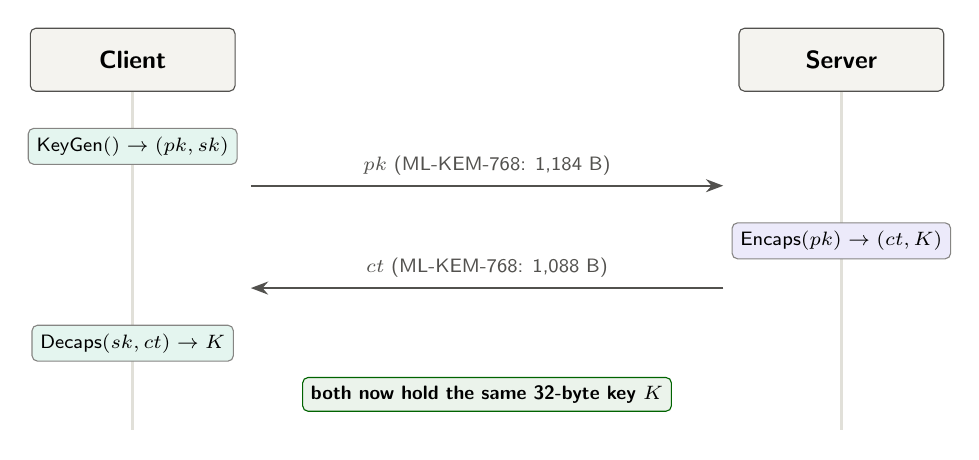
\begin{tikzpicture}
\node[party] (A) at (0,0) {Client};
\node[party] (B) at (9,0) {Server};
\draw[gridc,very thick] (A.south) -- ++(0,-4.3);
\draw[gridc,very thick] (B.south) -- ++(0,-4.3);
\node[op,fill=refc!12] (kg) at (0,-1.1) {$\mathsf{KeyGen}() \to (pk, sk)$};
\draw[msg] (1.5,-1.6) -- node[above,lbl]{$pk$ \hfill (ML-KEM-768: 1,184 B)} (7.5,-1.6);
\node[op,fill=optc!12] (en) at (9,-2.3) {$\mathsf{Encaps}(pk) \to (ct, K)$};
\draw[msg] (7.5,-2.9) -- node[above,lbl]{$ct$ \hfill (ML-KEM-768: 1,088 B)} (1.5,-2.9);
\node[op,fill=refc!12] (de) at (0,-3.6) {$\mathsf{Decaps}(sk, ct) \to K$};
\node[op,draw=good,fill=good!8,font=\sffamily\scriptsize\bfseries] at (4.5,-4.25) {both now hold the same 32-byte key $K$};
\end{tikzpicture}
\caption{One key exchange with a KEM: one message each way. E1 times each of the three boxes.}
\label{fig:kem}
\end{figure}

\textbf{How post-quantum KEMs get CCA security.} ML-KEM, HQC and FrodoKEM start from a public-key encryption scheme and apply a \key{Fujisaki–Okamoto-style transform}: $\mathsf{Decaps}$ decrypts, \emph{re-encrypts} and compares, returning a pseudo-random key on mismatch (implicit rejection). Classic McEliece uses its own Niederreiter-based construction, also with implicit rejection. The re-encryption is why \key{Decaps is usually the most expensive operation} for the lattice and HQC schemes (Section~\ref{sec:perop}).

\textbf{Why KEMs and not Diffie–Hellman?} Post-quantum cryptography has no efficient drop-in replacement for Diffie–Hellman's non-interactive "combine my secret with your public value". A KEM gives the same result, a shared key after one round trip, with a slightly different interface. NIST therefore standardised KEMs, and TLS 1.3 can carry them in its existing key-share messages.

% ------------------------------------------------------------------ 3
\sect{From Diffie–Hellman to a KEM}

\subsection{X25519 Diffie–Hellman}
X25519 (RFC 7748) works on Curve25519. A private key is a random 32-byte scalar $a$; the public key is $A = a\cdot G$. With the peer's public key $B$, both sides compute the same point $a\cdot B = b\cdot A = ab\cdot G$. TLS 1.3 uses it \key{ephemerally} (ECDHE): fresh key pairs on both sides for every handshake.

\begin{figure}[H]
\centering
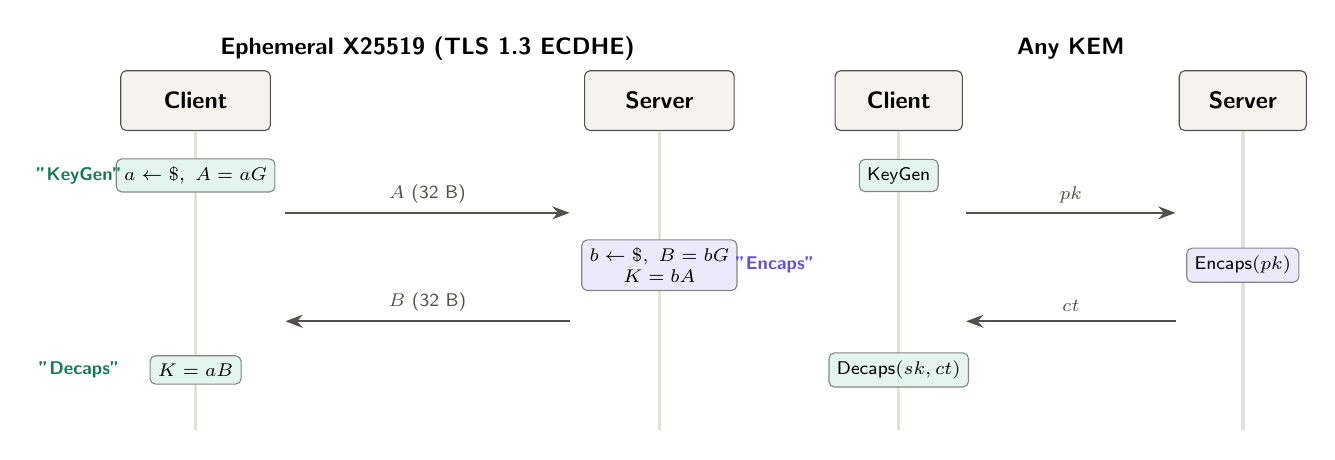
\begin{tikzpicture}[scale=0.95,transform shape]
% left: ECDHE
\node[font=\sffamily\bfseries\small] at (3.1,0.7) {Ephemeral X25519 (TLS 1.3 ECDHE)};
\node[party,minimum width=2cm] (A) at (0,0) {Client};
\node[party,minimum width=2cm] (B) at (6.2,0) {Server};
\draw[gridc,very thick] (A.south) -- ++(0,-4.0);
\draw[gridc,very thick] (B.south) -- ++(0,-4.0);
\node[op,fill=refc!12] at (0,-1.0) {$a \leftarrow \$,\ A = aG$};
\draw[msg] (1.2,-1.5) -- node[above,lbl]{$A$ (32 B)} (5.0,-1.5);
\node[op,fill=optc!12] at (6.2,-2.2) {$b \leftarrow \$,\ B = bG$\\$K = bA$};
\draw[msg] (5.0,-2.95) -- node[above,lbl]{$B$ (32 B)} (1.2,-2.95);
\node[op,fill=refc!12] at (0,-3.6) {$K = aB$};
% role labels
\node[lbl,text=refc!70!black,font=\sffamily\scriptsize\bfseries] at (-1.55,-1.0) {"KeyGen"};
\node[lbl,text=optc,font=\sffamily\scriptsize\bfseries] at (7.75,-2.2) {"Encaps"};
\node[lbl,text=refc!70!black,font=\sffamily\scriptsize\bfseries] at (-1.55,-3.6) {"Decaps"};
% right: KEM
\begin{scope}[xshift=9.4cm]
\node[font=\sffamily\bfseries\small] at (2.3,0.7) {Any KEM};
\node[party,minimum width=1.7cm] (C) at (0,0) {Client};
\node[party,minimum width=1.7cm] (D) at (4.6,0) {Server};
\draw[gridc,very thick] (C.south) -- ++(0,-4.0);
\draw[gridc,very thick] (D.south) -- ++(0,-4.0);
\node[op,fill=refc!12] at (0,-1.0) {$\mathsf{KeyGen}$};
\draw[msg] (0.9,-1.5) -- node[above,lbl]{$pk$} (3.7,-1.5);
\node[op,fill=optc!12] at (4.6,-2.2) {$\mathsf{Encaps}(pk)$};
\draw[msg] (3.7,-2.95) -- node[above,lbl]{$ct$} (0.9,-2.95);
\node[op,fill=refc!12] at (0,-3.6) {$\mathsf{Decaps}(sk,ct)$};
\end{scope}
\end{tikzpicture}
\caption{Ephemeral Diffie–Hellman already has the shape of a KEM: the client's key pair plays KeyGen, the server's key pair plus DH plays Encaps, and the client's DH plays Decaps.}
\label{fig:dh2kem}
\end{figure}

\subsection{Two ways to put X25519 next to the KEMs}
\begin{table}[H]
\centering\small
\begin{tabularx}{\linewidth}{@{}l>{\raggedright\arraybackslash}X>{\raggedright\arraybackslash}X@{}}
\toprule
KEM step & \key{X25519-ECDH} (plain, as in TLS 1.3) — \emph{our classical baseline} & \key{X25519-DHKEM} (RFC 9180, HPKE) \\
\midrule
KeyGen & $a \leftarrow \$$, $A = aG$ & same\\
Encaps$(A)$ & $b \leftarrow \$$, $B = bG$, $K = bA$; send $B$ & $(e, E)\leftarrow$ DeriveKeyPair; $K = \mathsf{ExtractAndExpand}(eA,\ E\|A)$; send $ct = E$\\
Decaps$(a, B)$ & $K = aB$ & $K = \mathsf{ExtractAndExpand}(aE,\ E\|A)$ \\
Cost & 2 key pairs + 2 DH per exchange & same + HKDF on both sides \\
Sizes & $pk$ = 32 B, "ct" = 32 B, $K$ = 32 B & same \\
\bottomrule
\end{tabularx}
\caption{X25519 measured as a KEM. We time both; the plain ECDH version is the fair baseline because TLS 1.3 does not use the HKDF wrapper (its own key schedule hashes $K$ later).}
\label{tab:dhkem}
\end{table}

\subsection{The hybrid X25519MLKEM768}
Deployed TLS combines both, so that the key stays safe if \emph{either} X25519 (quantum computers) or ML-KEM (new cryptanalysis) is broken:

\begin{figure}[H]
\centering
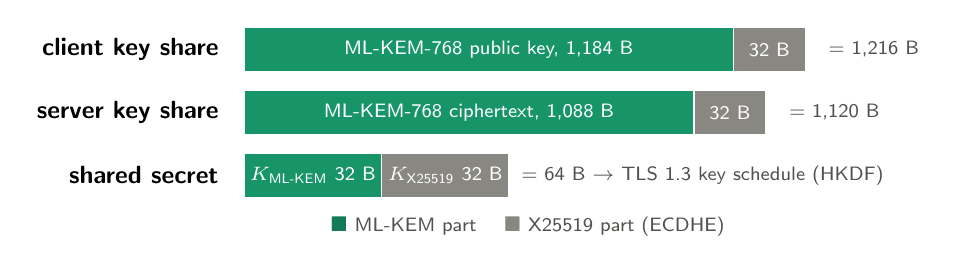
\begin{tikzpicture}[box/.style={draw=none,minimum height=0.55cm,font=\sffamily\scriptsize,text=white,inner sep=2pt}]
\node[font=\sffamily\small\bfseries,anchor=east] at (-0.2,0) {client key share};
\node[box,fill=refc!85!black,minimum width=6.2cm,anchor=west] (k1) at (0,0) {ML-KEM-768 public key, 1,184 B};
\node[box,fill=muted,minimum width=0.9cm,anchor=west] at (k1.east) {32 B};
\node[lbl,anchor=west] at (7.3,0) {= 1,216 B};
\node[font=\sffamily\small\bfseries,anchor=east] at (-0.2,-0.8) {server key share};
\node[box,fill=refc!85!black,minimum width=5.7cm,anchor=west] (c1) at (0,-0.8) {ML-KEM-768 ciphertext, 1,088 B};
\node[box,fill=muted,minimum width=0.9cm,anchor=west] at (c1.east) {32 B};
\node[lbl,anchor=west] at (6.8,-0.8) {= 1,120 B};
\node[font=\sffamily\small\bfseries,anchor=east] at (-0.2,-1.6) {shared secret};
\node[box,fill=refc!85!black,minimum width=1.6cm,anchor=west] (s1) at (0,-1.6) {$K_\text{ML-KEM}$ 32 B};
\node[box,fill=muted,minimum width=1.6cm,anchor=west] (s2) at (s1.east) {$K_\text{X25519}$ 32 B};
\node[lbl,anchor=west] at (3.4,-1.6) {= 64 B $\to$ TLS 1.3 key schedule (HKDF)};
\node[lbl] at (3.6,-2.25) {\textcolor{refc!70!black}{$\blacksquare$} ML-KEM part \quad \textcolor{muted}{$\blacksquare$} X25519 part (ECDHE)};
\end{tikzpicture}
\caption{X25519MLKEM768 (IETF \texttt{draft-ietf-tls-ecdhe-mlkem}) concatenates both key shares and both secrets. The sizes are exactly those measured in E1.}
\label{fig:hybrid}
\end{figure}

% ------------------------------------------------------------------ 4
\sect{Experimental setup and our choices}

\subsection{Machines}
\begin{table}[H]
\centering\small
\begin{tabular}{lll}
\toprule
 & Apple M4 (ARM64) & Intel i7-1185G7 (x86-64) \\
\midrule
CPU & Apple M4 & Intel i7-1185G7 \\
cores & 10 & 8 \\
environment & Docker Desktop (Linux VM) & WSL2 (Ubuntu 24.04) \\
kernel & 7.0.14-linuxkit & 6.18.40.1-microsoft-standard-WSL2 \\
compiler & GCC 13.3.0 (Ubuntu 24.04) & GCC 13.3.0 (Ubuntu 24.04) \\
liboqs & 0.16.0 & 0.16.0 \\
OpenSSL & 3.5.8 & 3.5.8 \\
timer (MHz) & 24.000 & 1857.904 \\
core clock at start (GHz) & 4.395 & 3.890 \\
timed calls per op & 1000 & 1000 \\
McEliece keygens & 100 & 100 \\
cooldown (s) & 30 & 30 \\
warm-up (ms) & 200 & 200 \\
code commit & 124a4d6 & e144cb6 \\
\bottomrule
\end{tabular}

\caption{The two machines, read from the metadata header of each results file. Both run the same Ubuntu 24.04 userland, compiler and library versions; only the CPU differs.}
\end{table}

\subsection{Implementations and builds}

\begin{figure}[H]
\centering
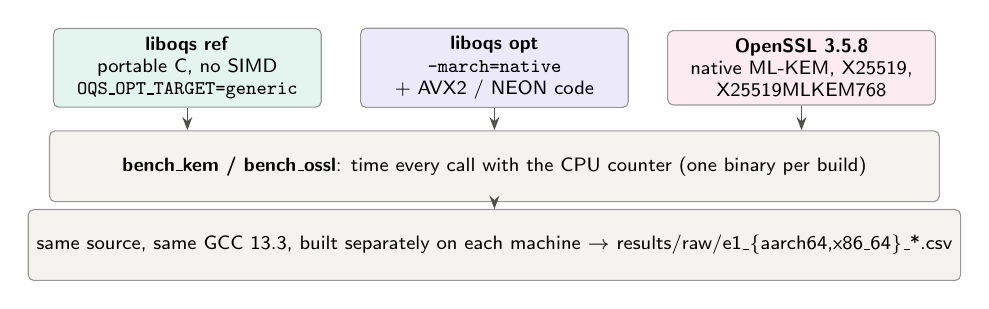
\begin{tikzpicture}[blk/.style={draw=ink2!60,rounded corners=2pt,font=\sffamily\scriptsize,align=center,minimum height=0.9cm,inner sep=3pt,fill=white}]
\node[blk,minimum width=3.4cm,fill=refc!12] (ref) at (0,0) {\textbf{liboqs ref}\\portable C, no SIMD\\\texttt{OQS\_OPT\_TARGET=generic}};
\node[blk,minimum width=3.4cm,fill=optc!12] (opt) at (3.9,0) {\textbf{liboqs opt}\\\texttt{-march=native}\\+ AVX2 / NEON code};
\node[blk,minimum width=3.4cm,fill=osslc!15] (os) at (7.8,0) {\textbf{OpenSSL 3.5.8}\\native ML-KEM, X25519,\\X25519MLKEM768};
\node[blk,minimum width=11.3cm,fill=wash] (b) at (3.9,-1.25) {\textbf{bench\_kem / bench\_ossl}: time every call with the CPU counter (one binary per build)};
\node[blk,minimum width=11.3cm,fill=wash] (c) at (3.9,-2.25) {same source, same GCC 13.3, built separately on each machine $\to$ results/raw/e1\_\{aarch64,x86\_64\}\_*.csv};
\draw[-{Stealth},ink2] (ref) -- (b.north -| ref);
\draw[-{Stealth},ink2] (opt) -- (b.north -| opt);
\draw[-{Stealth},ink2] (os) -- (b.north -| os);
\draw[-{Stealth},ink2] (b) -- (c);
\end{tikzpicture}
\caption{Three builds per machine. ref vs opt isolates what hand-optimised code adds; OpenSSL is the implementation that TLS deployments actually run.}
\end{figure}

\begin{table}[H]
\centering\small
\begin{tabular}{lccl}
\toprule
KEM family & x86-64: AVX2 code & ARM64: NEON code & consequence\\
\midrule
ML-KEM (mlkem-native) & \checkmark & \checkmark & opt faster on both\\
FrodoKEM & \checkmark & -- & opt = ref on M4\\
Classic McEliece & \checkmark & -- & opt = ref on M4\\
HQC & -- & -- & opt = ref (only compiler gains)\\
\bottomrule
\end{tabular}
\caption{Optimised code available in liboqs 0.16.0. This table explains most of the cross-machine differences in Section~\ref{sec:arch}.}
\label{tab:simd}
\end{table}

\subsection{Measurement method}
\begin{figure}[H]
\centering
\begin{tikzpicture}[st/.style={draw=ink2!60,rounded corners=2pt,font=\sffamily\scriptsize,align=center,minimum height=1.25cm,text width=2.05cm,fill=white,inner sep=2pt},
  arr/.style={-{Stealth},thick,muted}]
\node[st,fill=wash] (s1) at (0,0) {\textbf{calibrate}\\ticks $\to$ ns once per run (5×200\,ms)};
\node[st,fill=wash] (s2) at (2.45,0) {\textbf{warm up}\\200\,ms busy loop + 10\% of calls};
\node[st,fill=mfour!10] (s3) at (4.9,0) {\textbf{time}\\1,000 calls each (McEliece keygen: 100)};
\node[st,fill=wash] (s4) at (7.35,0) {\textbf{core clock}\\add-chain estimate before and after};
\node[st,fill=wash] (s5) at (9.8,0) {\textbf{summarise}\\median, IQR, stack peak, sizes};
\node[st,fill=wash] (s6) at (12.25,0) {\textbf{cool down}\\30\,s, next KEM};
\foreach \a/\b in {s1/s2,s2/s3,s3/s4,s4/s5,s5/s6} \draw[arr] (\a) -- (\b);
\end{tikzpicture}
\caption{E1 pipeline, repeated for every KEM, build and operation (90 rows per machine). The process is pinned to one core.}
\end{figure}

\begin{table}[H]
\centering\small
\begin{tabularx}{\linewidth}{@{}>{\raggedright\arraybackslash}p{4.2cm}>{\raggedright\arraybackslash}X@{}}
\toprule
Choice & Why \\
\midrule
Time every call individually, report the \key{median} and IQR & Robust to interrupts and the occasional slow call; the IQR shows stability. \\
Hardware counter (TSC on x86, 24\,MHz CNTVCT on ARM) & Readable inside Docker and WSL2, where the real cycle counter is not; converted to ns once per run. \\
200\,ms warm-up & Measured: the M4 needs $\sim$90\,ms to ramp from 2.0 to 4.4\,GHz after idling. \\
Core-clock estimate (chain of dependent adds) & Lets us report \key{core cycles}, comparable with papers, despite turbo and AVX frequency changes. \\
30\,s cooldown between KEMs & The MacBook Air is fanless: without pauses later KEMs would run on a hotter, slower chip. \\
100 McEliece keygens & Its key generation retries until a random matrix works; 20 samples gave unstable medians. \\
ref + opt builds of the same library & Separates algorithm cost from implementation effort. \\
Two architectures, same software & ARM64 vs x86-64 with identical code, compiler and versions. \\
Full exchange = keygen + encaps + decaps & One complete key agreement, comparable across KEMs and with ECDH. \\
\bottomrule
\end{tabularx}
\caption{Methodological choices and their justification.}
\end{table}

% ------------------------------------------------------------------ 5
\sect{E4: correctness}
Before comparing speed, we checked that every implementation computes the right answer.

\begin{table}[H]
\centering\small
\begin{tabularx}{\linewidth}{@{}l>{\raggedright\arraybackslash}X l@{}}
\toprule
Check & What it proves & Applies to\\
\midrule
KAT & Deterministic output hashed and compared with the reference hash shipped by liboqs & all 12 KEMs, both builds\\
NIST ACVP & keyGen, encapsulation and decapsulation vectors from NIST's FIPS 203 validation suite & ML-KEM (60 per level)\\
Round trips & Random keygen $\to$ encaps $\to$ decaps gives the same key (50, McEliece 3) & all, both builds\\
Cross-build & Key from one build, encapsulate with the other, decapsulate with the first (both ways) & all\\
Interop & liboqs $\leftrightarrow$ OpenSSL 3.5 native ML-KEM, both directions & ML-KEM\\
\bottomrule
\end{tabularx}
\caption{The five E4 checks.}
\end{table}

\begin{figure}[H]
\centering
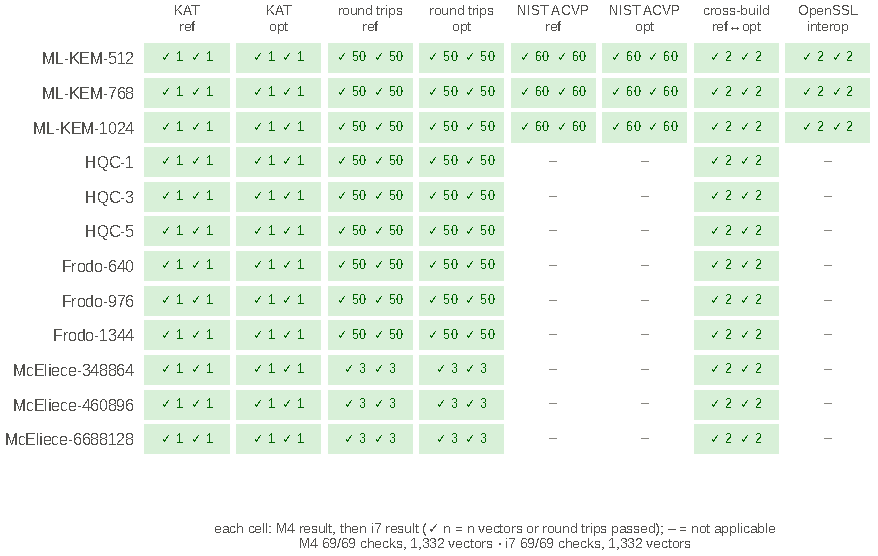
\includegraphics[width=\linewidth]{fig/e4_matrix.pdf}
\caption{E4 results. Every applicable check passes on both machines, \eFourVectors{} vectors and round trips each.}
\end{figure}

\begin{takeaway}
\begin{itemize}
\item All \eFourChecks{} checks pass on ARM64 and x86-64: \key{the optimised AVX2/NEON code computes exactly what the portable code does}, so E1 compares like with like.
\item ML-KEM in liboqs matches NIST's official FIPS 203 vectors and interoperates with OpenSSL's independent implementation.
\item Limitation: ACVP's key-check groups (FIPS 203 input validation) are not exposed by the liboqs API and are skipped, as in liboqs' own test.
\end{itemize}
\end{takeaway}

% ------------------------------------------------------------------ 6
\clearpage
\sect{E1: performance}
\emph{Best build} below means liboqs \texttt{opt} for the post-quantum KEMs and OpenSSL for X25519 and the hybrid. Times are medians per call; a full exchange is the sum of the three medians.

\subsection{Sizes: what goes over the wire}
\begin{figure}[H]
\centering
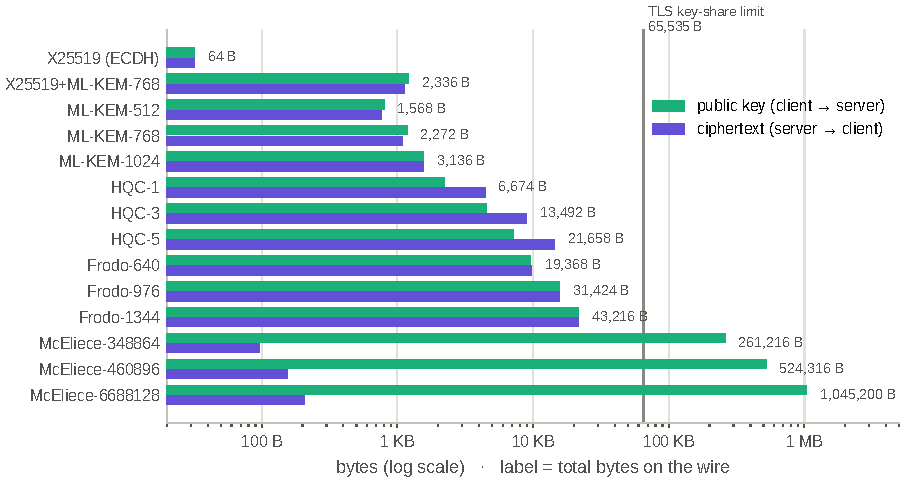
\includegraphics[width=\linewidth]{fig/sizes.pdf}
\caption{Public key and ciphertext per KEM (identical on both machines). McEliece's public key does not fit in a TLS key share.}
\label{fig:sizes}
\end{figure}

\begin{table}[H]
\centering\small
\begin{tabular}{lrrrrrr}
\toprule
KEM & level & public key & secret key & ciphertext & shared secret & on wire \\
\midrule
X25519 (ECDH) & – & 32 & 32 & 32 & 32 & 64 \\
ML-KEM-512 & 1 & 800 & 1,632 & 768 & 32 & 1,568 \\
ML-KEM-768 & 3 & 1,184 & 2,400 & 1,088 & 32 & 2,272 \\
ML-KEM-1024 & 5 & 1,568 & 3,168 & 1,568 & 32 & 3,136 \\
HQC-1 & 1 & 2,241 & 2,321 & 4,433 & 32 & 6,674 \\
HQC-3 & 3 & 4,514 & 4,602 & 8,978 & 32 & 13,492 \\
HQC-5 & 5 & 7,237 & 7,333 & 14,421 & 32 & 21,658 \\
Frodo-640 & 1 & 9,616 & 19,888 & 9,752 & 16 & 19,368 \\
Frodo-976 & 3 & 15,632 & 31,296 & 15,792 & 24 & 31,424 \\
Frodo-1344 & 5 & 21,520 & 43,088 & 21,696 & 32 & 43,216 \\
McEliece-348864 & 1 & 261,120 & 6,492 & 96 & 32 & 261,216 \\
McEliece-460896 & 3 & 524,160 & 13,608 & 156 & 32 & 524,316 \\
McEliece-6688128 & 5 & 1,044,992 & 13,932 & 208 & 32 & 1,045,200 \\
X25519+ML-KEM-768 & – & 1,216 & – & 1,120 & 64 & 2,336 \\
\bottomrule
\end{tabular}

\caption{Sizes in bytes, as reported by the implementations; they match the specifications exactly.}
\end{table}

\begin{takeaway}
\begin{itemize}
\item ML-KEM: \key{25–49× X25519's 64 bytes} (35× at level 3), still only 1.5–3\,KB. HQC is 4–7× ML-KEM, FrodoKEM 12–14×.
\item Classic McEliece is the opposite trade: \key{the smallest ciphertext (96–208\,B) but 0.26–1\,MB public keys}, beyond the 65,535-byte TLS limit.
\end{itemize}
\end{takeaway}

\subsection{The full exchange}
\begin{figure}[H]
\centering
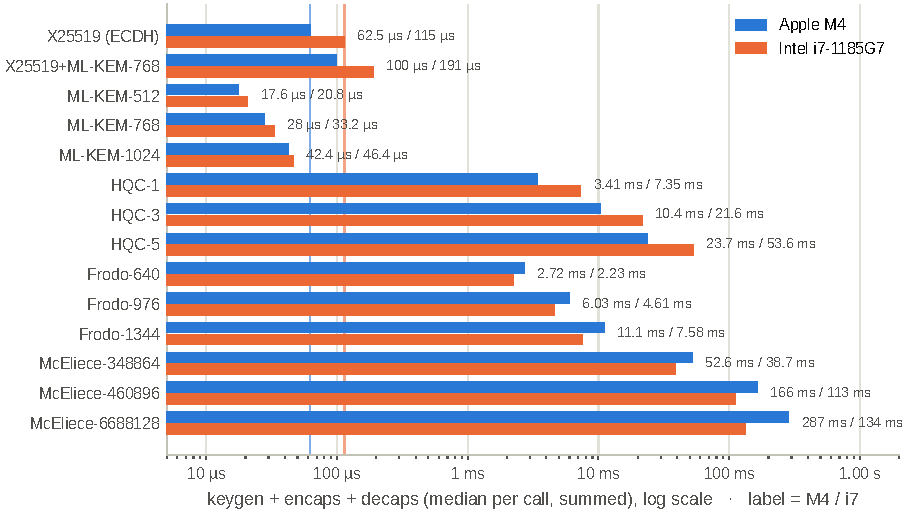
\includegraphics[width=\linewidth]{fig/full_exchange.pdf}
\caption{Compute for one complete key exchange, best build. The thin vertical lines mark X25519 ECDH on each machine.}
\label{fig:full}
\end{figure}

\begin{figure}[H]
\centering
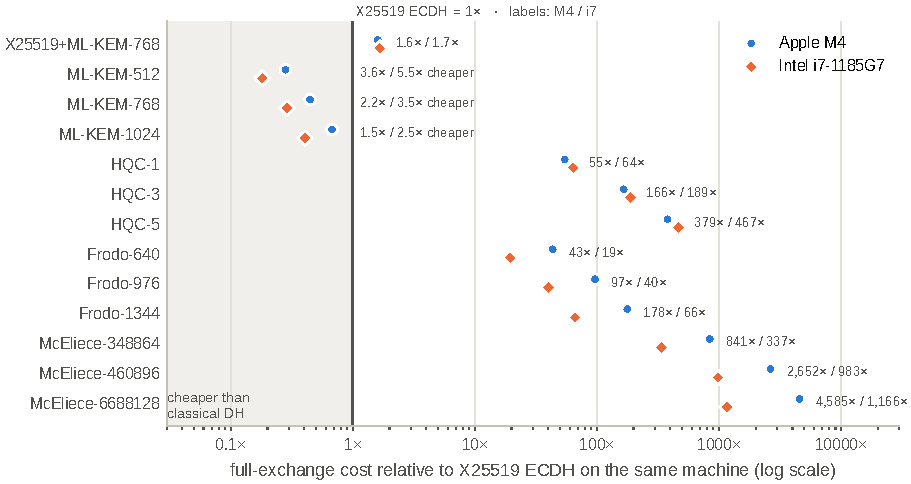
\includegraphics[width=\linewidth]{fig/relative_to_x25519.pdf}
\caption{The same, relative to X25519 ECDH on the same machine (shaded = cheaper than classical DH).}
\label{fig:rel}
\end{figure}

\begin{takeaway}
\begin{itemize}
\item \key{ML-KEM is cheaper than classical X25519} at every level: level 3 is \invMmlkemIII× (M4) and \invImlkemIII× (i7) cheaper; level 1 up to \invImlkemI×.
\item The \key{hybrid costs \relMhybrid–\relIhybrid× X25519}: adding post-quantum security to today's TLS is cheap in compute.
\item HQC (\relMhqcI–\relIhqcI× at level 1), FrodoKEM (\relIfrodoI–\relMfrodoI×) and McEliece (\relImceI–\relMmceI×) cost one to three orders of magnitude more.
\end{itemize}
\end{takeaway}

\subsection{Per operation}
\label{sec:perop}
\begin{figure}[H]
\centering
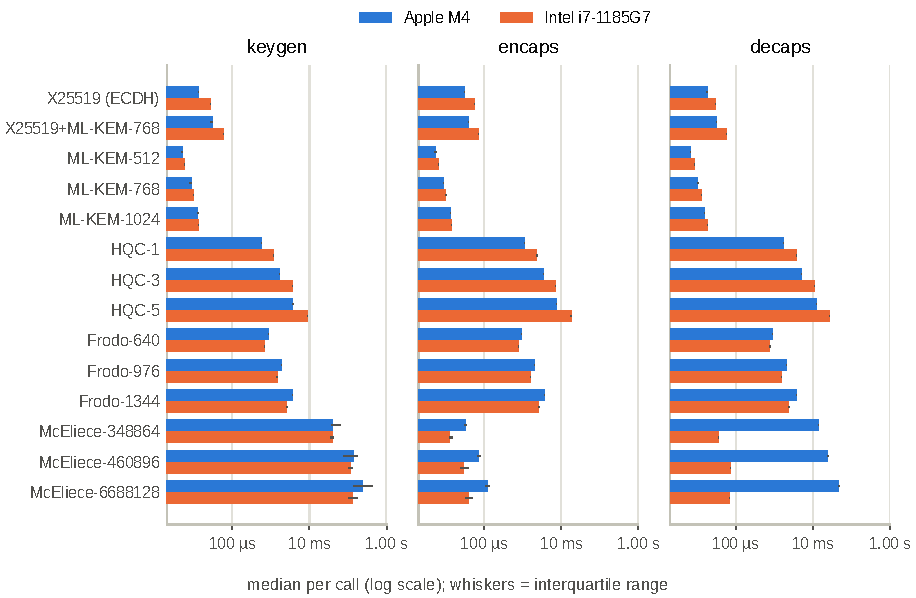
\includegraphics[width=\linewidth]{fig/per_op.pdf}
\caption{Median per call for each operation, best build, both machines.}
\label{fig:perop}
\end{figure}

\begin{itemize}
\item \key{ML-KEM, HQC:} decaps $>$ encaps $>$ keygen, because of the re-encryption check. HQC follows the 1:2:3 ratio of its specification.
\item \key{FrodoKEM:} all three about equal, since generating the large matrix from a seed dominates every operation.
\item \key{Classic McEliece:} keygen 39–239\,ms (it retries until a random matrix gives a valid key), encaps 13–121\,µs (very fast), decaps 37–73\,µs with AVX2 but 14–48\,ms without. The work sits with whoever makes the key.
\item \key{X25519:} encaps $\approx$ keygen + decaps, since the server does both a key pair and a DH.
\end{itemize}

\subsection{The cost/size trade-off}
\begin{figure}[H]
\centering
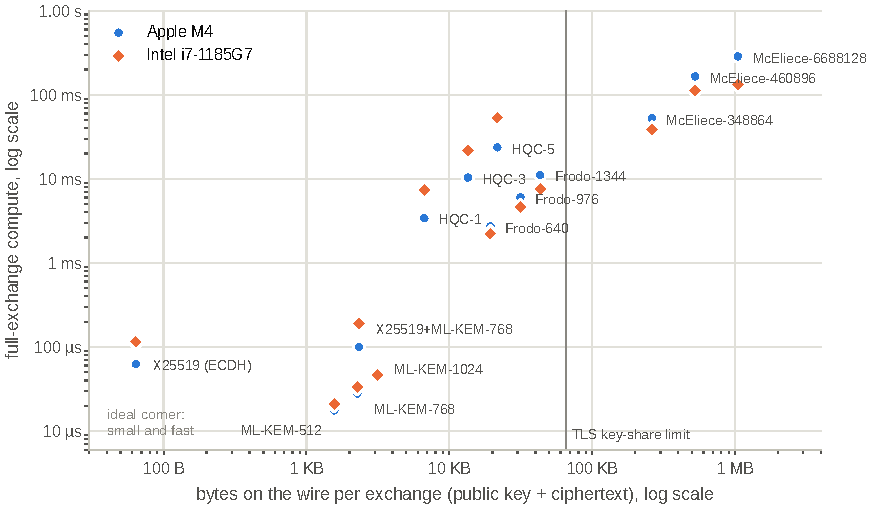
\includegraphics[width=\linewidth]{fig/tradeoff.pdf}
\caption{Compute vs. bytes on the wire, per full exchange. Bottom-left is best.}
\label{fig:tradeoff}
\end{figure}

\begin{takeaway}
\begin{itemize}
\item \key{ML-KEM is the only KEM in the "small and fast" corner}; X25519 is smaller but slower.
\item FrodoKEM and HQC cost both more bytes and more compute; McEliece trades huge keys for its tiny ciphertext.
\item The chart is the core result of RQ1: the conservative choices are expensive \emph{in both dimensions}.
\end{itemize}
\end{takeaway}

\subsection{Security level scaling}
\begin{figure}[H]
\centering
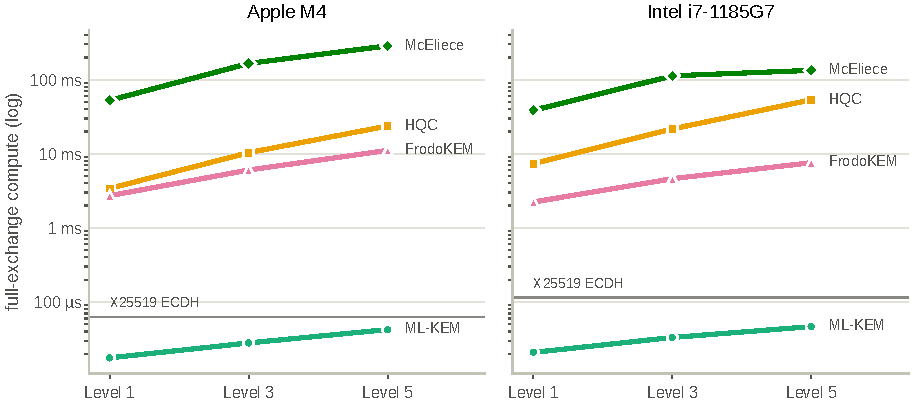
\includegraphics[width=\linewidth]{fig/levels.pdf}
\caption{Full-exchange compute from NIST level 1 to 5 (log scale). ML-KEM stays below X25519 even at level 5.}
\label{fig:levels}
\end{figure}

\begin{itemize}
\item From level 1 to 5: ML-KEM ×2.2–2.4, HQC ×7, FrodoKEM ×3.4–4.1, McEliece ×3.5–5.4.
\item \key{Why ML-KEM stays cheap:} its arithmetic is on 12-bit numbers (mod 3329), 8–16 per SIMD instruction, multiplied with the NTT. X25519 needs about 2,500 sequential 255-bit multiplications per operation (58k cycles per key pair on the M4). Large keys do not imply heavy computation.
\end{itemize}

\subsection{Optimised vs. portable code}
\begin{figure}[H]
\centering
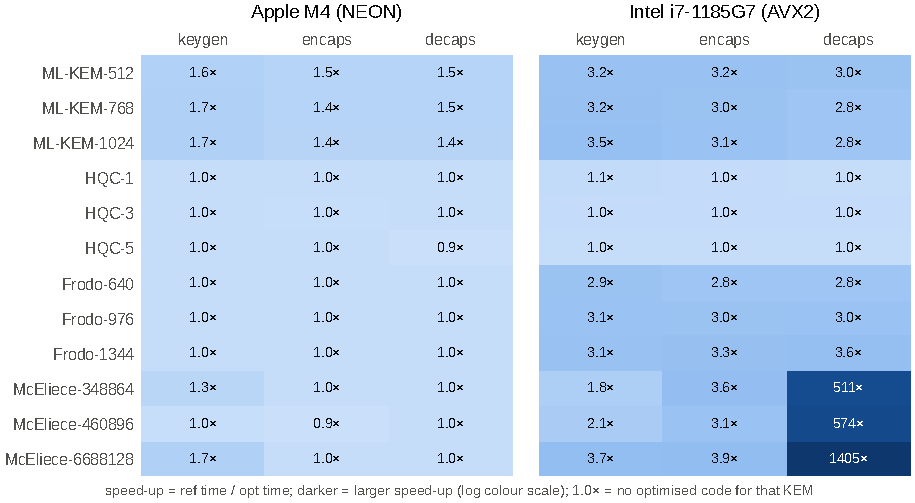
\includegraphics[width=\linewidth]{fig/speedup.pdf}
\caption{Speed-up of the optimised build over the portable one.}
\label{fig:speedup}
\end{figure}

\begin{itemize}
\item \key{AVX2 (i7):} ML-KEM and FrodoKEM about 3×; McEliece decaps \key{510–1,400×} (bitsliced decoding instead of portable C).
\item \key{NEON (M4):} only ML-KEM has NEON code, 1.4–1.7×; everything else is 1.0× (Table~\ref{tab:simd}). The McEliece keygen values (0.95–1.7×) are noise from its retry loop.
\item \key{HQC:} 1.0× on both, since liboqs 0.16 ships no AVX2 HQC. The HQC team's own AVX2 code (76k/150k/353k cycles at level 1 in its specification) is 33–49× faster than what we measured, so HQC's large gap to ML-KEM is partly an implementation gap.
\end{itemize}

\subsection{ARM64 vs. x86-64}
\label{sec:arch}
\begin{figure}[H]
\centering
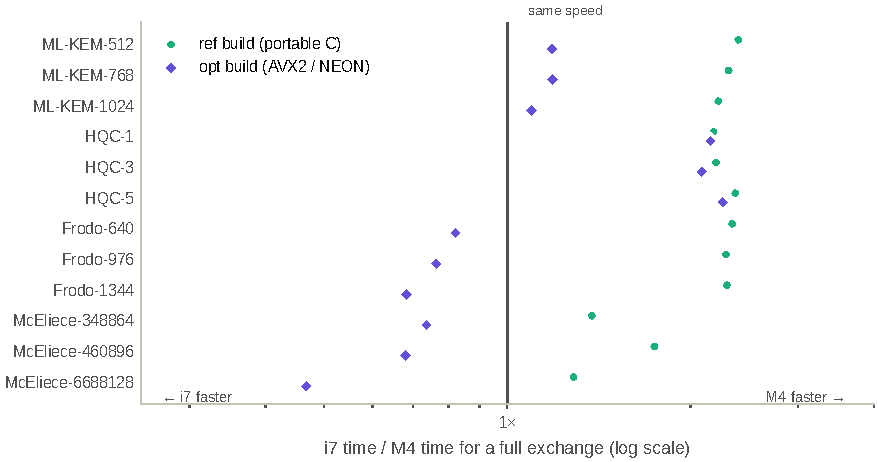
\includegraphics[width=\linewidth]{fig/machine_ratio.pdf}
\caption{i7 time divided by M4 time for a full exchange. Right of 1×: the M4 is faster.}
\label{fig:arch}
\end{figure}

\begin{figure}[H]
\centering
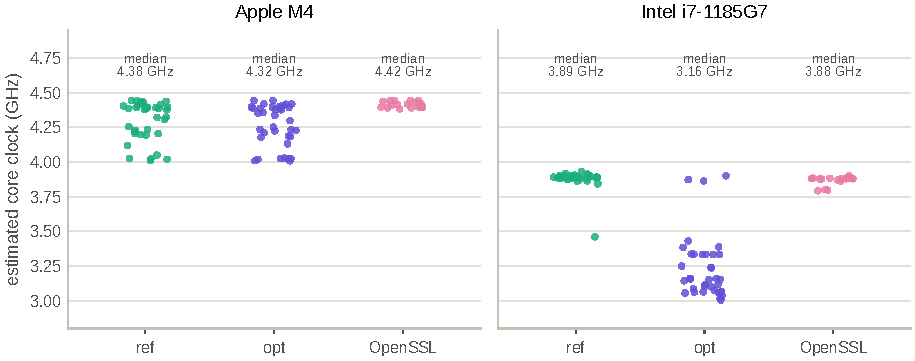
\includegraphics[width=\linewidth]{fig/clock.pdf}
\caption{Core clock estimated around every timed loop. The i7 drops to $\sim$3.2\,GHz while running AVX2 code; the M4 stays at 4.0–4.44\,GHz (the lowest points are the longest loops, where the fanless Air throttles slightly).}
\label{fig:clock}
\end{figure}

\begin{takeaway}
\begin{itemize}
\item \key{On the same portable code the M4 is about 2.2× faster} (wider core, higher clock).
\item \key{With optimised code the winner depends on what exists:} ML-KEM about equal (i7 1.1–1.2× slower), FrodoKEM and McEliece faster on the i7 (AVX2 code, no NEON code).
\item \key{The i7 lowers its clock for AVX2 code} (3.9 $\to$ 3.2\,GHz). In core cycles AVX2 ML-KEM-768 is 3.3–3.6× cheaper than portable (published for Kyber: 3.5–5.2×); in time the gain shrinks to 2.8–3.2×.
\end{itemize}
\end{takeaway}

\subsection{The classical baseline and the hybrid}
\begin{figure}[H]
\centering
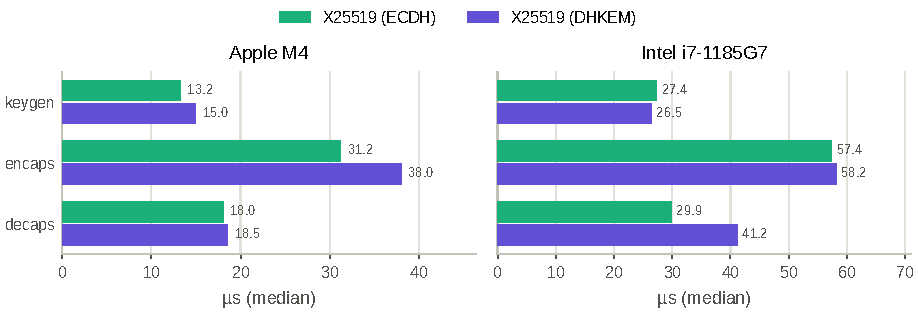
\includegraphics[width=\linewidth]{fig/ecdh_vs_dhkem.pdf}
\caption{Plain X25519 ECDH vs. the same curve wrapped as a KEM (DHKEM, RFC 9180).}
\label{fig:dhkem}
\end{figure}

\begin{figure}[H]
\centering
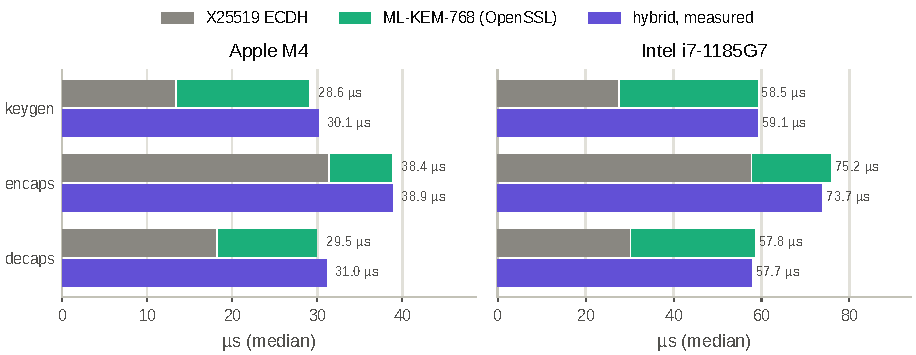
\includegraphics[width=\linewidth]{fig/hybrid.pdf}
\caption{Measured hybrid vs. the sum of its parts (X25519 ECDH + OpenSSL's ML-KEM-768).}
\label{fig:hybridm}
\end{figure}

\begin{itemize}
\item The \key{DHKEM wrapper adds 10–14\%} to a full exchange (one HKDF per side), so plain ECDH is the fairer baseline. The i7's DHKEM decaps row is noisy (IQR 28\%).
\item \key{The hybrid costs its two parts added together} (within 5\%): combining them is essentially free.
\item OpenSSL's ML-KEM keygen is 1.8–3.2× slower than liboqs \texttt{opt}, which matters for the hybrid's client side.
\end{itemize}

\subsection{Memory: stack use}
\begin{figure}[H]
\centering
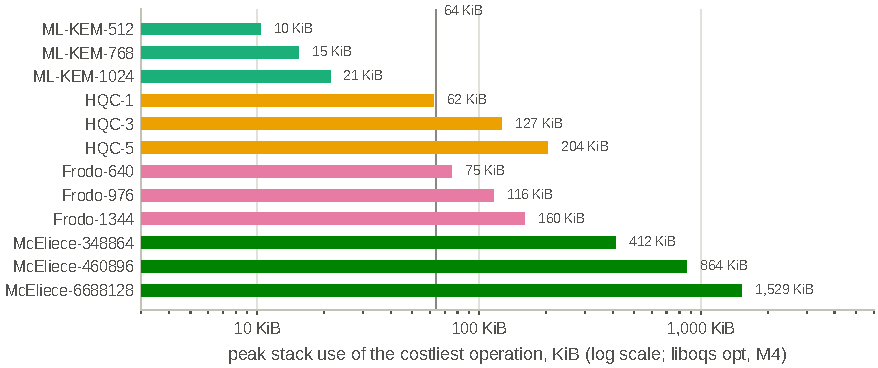
\includegraphics[width=\linewidth]{fig/stack.pdf}
\caption{Peak stack of the most demanding operation (liboqs opt, M4).}
\label{fig:stack}
\end{figure}
\key{ML-KEM fits in 10–21\,KiB}. HQC and FrodoKEM need 60–200\,KiB, and McEliece 0.4–1.5\,MiB, which rules it out of small embedded devices and constrained threads.

\subsection{Validation against published results}
\begin{table}[H]
\centering\small
\begin{tabular}{lrrrrl}
\toprule
 & keygen & encaps & decaps & ours/pub. & published on \\
\midrule
ML-KEM-768, AVX2 & 33k / 53k & 34k / 68k & 44k / 53k & 0.65 & Kyber R3 spec, Haswell \\
ML-KEM-768, portable & 119k / 199k & 120k / 235k & 144k / 275k & 0.54 & Kyber R3 spec, Haswell \\
HQC-1, portable & 3.6M / 4.6M & 7.3M / 9.1M & 11.5M / 13.9M & 0.81 & HQC spec 2025, i7-11850H \\
Frodo-640, AVX2 & 2.1M / 4.0M & 2.4M / 4.2M & 2.4M / 4.1M & 0.56 & FrodoKEM spec, Skylake \\
McEliece-348864, AVX2 & 120.0M / 46.5M & 41k / 44k & 115k / 134k & 1.46 & McEliece R3, Haswell \\
\bottomrule
\end{tabular}

\caption{Our i7 core cycles (estimated) vs. the designers' published cycle counts ("ours / published"). Published values use turbo off on older Intel cores, and the Kyber numbers are for the Round-3 code, the pre-standard version of ML-KEM.}
\label{tab:pub}
\end{table}
\begin{itemize}
\item \key{Agreement where the code is the same:} HQC (same portable code, same Intel generation) within 20\%; McEliece encaps/decaps within 7–14\%.
\item \key{Fewer cycles for ML-KEM and FrodoKEM:} newer, faster implementations (mlkem-native in liboqs; 4-way SHAKE) on a newer core.
\item \key{Open discrepancy:} McEliece-348864 keygen at 120M cycles is 2.6× the published 46.5M, with 100 samples. To be investigated.
\end{itemize}

% ------------------------------------------------------------------ 7
\sect{Findings, limitations and next steps}

\begin{takeaway}[Key findings]
\begin{enumerate}
\item All implementations are correct on both architectures (E4), including against NIST's FIPS 203 vectors.
\item \key{ML-KEM is cheaper than classical X25519} in compute (\invMmlkemIII–\invImlkemIII× at level 3); its cost is bandwidth (35× more bytes), not CPU.
\item The deployed hybrid costs \relMhybrid–\relIhybrid× X25519, exactly its parts added together.
\item Conservative alternatives cost 1–3 orders of magnitude more compute \emph{and} more bytes: HQC 55–64×, FrodoKEM 19–43×, McEliece 337–841× at level 1.
\item \key{Implementation matters as much as the algorithm:} AVX2 changes McEliece decaps by up to 1,400×, missing NEON code makes the M4 slower than an older i7, and HQC lacks optimised code in liboqs.
\end{enumerate}
\end{takeaway}

\textbf{Limitations}
\begin{itemize}
\item Both machines run Linux in a VM (Docker Desktop, WSL2); per-call overhead is small for these CPU-bound loops but not zero.
\item The ARM timer ticks every 41.7\,ns, i.e.\ 0.4–0.8\% of the fastest operations (5–10\,µs); the median of 1,000 calls averages this out.
\item The i7's tick-to-ns conversion differed by 2.4\% between the main run and the appended X25519-ECDH rows (WSL2 clock); core-cycle values are unaffected.
\item McEliece keygen timing varies a lot by nature (IQR 55–120\%).
\item One laptop per architecture; results describe these CPUs, not every ARM or x86 chip.
\end{itemize}

\textbf{Next (Part 2):} E2 measures what these costs mean inside real TLS 1.3 handshakes under network delay and loss; E3 tests the implementations for timing side channels (dudect, Valgrind, KyberSlash).

% ------------------------------------------------------------------ appendix
\appendix
\sect{Full E1 results}
\begin{table}[H]
\centering\scriptsize\setlength{\tabcolsep}{4pt}
\begin{tabular}{llrrrrrrr}
\toprule
KEM & build & keygen & encaps & decaps & kg cyc & enc cyc & dec cyc & IQR \\
\midrule
X25519 (ECDH) & openssl & 13.2\,µs & 31.2\,µs & 18\,µs & 58k & 138k & 80k & 4\% \\
X25519+ML-KEM-768 & openssl & 30.1\,µs & 38.9\,µs & 31\,µs & 133k & 172k & 138k & 8\% \\
X25519 (DHKEM) & openssl & 15\,µs & 38\,µs & 18.5\,µs & 66k & 167k & 82k & 9\% \\
\midrule
ML-KEM-512 & ref & 8.54\,µs & 8.33\,µs & 9.96\,µs & 37k & 36k & 42k & 2\% \\
ML-KEM-512 & opt & 5.21\,µs & 5.67\,µs & 6.71\,µs & 23k & 25k & 29k & 9\% \\
ML-KEM-512 & openssl & 9.62\,µs & 5.33\,µs & 8.79\,µs & 42k & 23k & 39k & 9\% \\
ML-KEM-768 & ref & 14.5\,µs & 13\,µs & 15.2\,µs & 64k & 57k & 67k & 8\% \\
ML-KEM-768 & opt & 8.5\,µs & 8.96\,µs & 10.5\,µs & 37k & 39k & 46k & 9\% \\
ML-KEM-768 & openssl & 15.3\,µs & 7.17\,µs & 11.5\,µs & 67k & 32k & 51k & 10\% \\
ML-KEM-1024 & ref & 22.4\,µs & 19.7\,µs & 22.5\,µs & 98k & 86k & 99k & 8\% \\
ML-KEM-1024 & opt & 12.8\,µs & 13.7\,µs & 15.9\,µs & 57k & 60k & 69k & 1\% \\
ML-KEM-1024 & openssl & 23.2\,µs & 9.33\,µs & 15.2\,µs & 102k & 41k & 67k & 10\% \\
\midrule
HQC-1 & ref & 561\,µs & 1.12\,ms & 1.71\,ms & 2,490k & 4,996k & 7,548k & 1\% \\
HQC-1 & opt & 561\,µs & 1.12\,ms & 1.72\,ms & 2,492k & 4,929k & 7,208k & 1\% \\
HQC-3 & ref & 1.69\,ms & 3.36\,ms & 5.09\,ms & 7,475k & 14.8M & 21.4M & 1\% \\
HQC-3 & opt & 1.69\,ms & 3.53\,ms & 5.14\,ms & 6,971k & 14.9M & 20.7M & 1\% \\
HQC-5 & ref & 3.68\,ms & 7.44\,ms & 11.2\,ms & 15.5M & 29.9M & 44.9M & 1\% \\
HQC-5 & opt & 3.72\,ms & 7.56\,ms & 12.4\,ms & 15.0M & 30.3M & 52.3M & 1\% \\
\midrule
Frodo-640 & ref & 862\,µs & 923\,µs & 917\,µs & 3,804k & 4,088k & 3,883k & 1\% \\
Frodo-640 & opt & 873\,µs & 927\,µs & 918\,µs & 3,837k & 4,038k & 3,947k & 1\% \\
Frodo-976 & ref & 1.93\,ms & 2.09\,ms & 2.07\,ms & 8,594k & 8,821k & 8,403k & 1\% \\
Frodo-976 & opt & 1.91\,ms & 2.07\,ms & 2.05\,ms & 8,391k & 8,285k & 8,269k & 1\% \\
Frodo-1344 & ref & 3.49\,ms & 3.81\,ms & 3.72\,ms & 14.6M & 15.7M & 15.0M & 1\% \\
Frodo-1344 & opt & 3.57\,ms & 3.79\,ms & 3.75\,ms & 14.9M & 15.3M & 15.7M & 1\% \\
\midrule
McEliece-348864 & ref & 51.8\,ms & 32.5\,µs & 13.6\,ms & 228.1M & 140k & 60.0M & 72\% \\
McEliece-348864 & opt & 38.6\,ms & 32.6\,µs & 13.9\,ms & 163.2M & 141k & 61.4M & 65\% \\
McEliece-460896 & ref & 134\,ms & 66.2\,µs & 24.6\,ms & 566.0M & 290k & 107.9M & 94\% \\
McEliece-460896 & opt & 141\,ms & 73.8\,µs & 24.7\,ms & 596.6M & 326k & 109.9M & 68\% \\
McEliece-6688128 & ref & 413\,ms & 121\,µs & 47.6\,ms & 1,737.4M & 484k & 205.2M & 119\% \\
McEliece-6688128 & opt & 239\,ms & 121\,µs & 47.7\,ms & 1,009.6M & 486k & 202.7M & 123\% \\
\bottomrule
\end{tabular}

\caption{Apple M4: medians per call, estimated core cycles, and the largest relative IQR of the three operations.}
\end{table}
\begin{table}[H]
\centering\scriptsize\setlength{\tabcolsep}{4pt}
\begin{tabular}{llrrrrrrr}
\toprule
KEM & build & keygen & encaps & decaps & kg cyc & enc cyc & dec cyc & IQR \\
\midrule
X25519 (ECDH) & openssl & 27.4\,µs & 57.4\,µs & 29.9\,µs & 104k & 218k & 114k & 1\% \\
X25519+ML-KEM-768 & openssl & 59.1\,µs & 73.7\,µs & 57.7\,µs & 231k & 286k & 224k & 1\% \\
X25519 (DHKEM) & openssl & 26.5\,µs & 58.2\,µs & 41.2\,µs & 103k & 226k & 159k & 28\% \\
\midrule
ML-KEM-512 & ref & 18.5\,µs & 20.7\,µs & 25.1\,µs & 72k & 80k & 98k & 1\% \\
ML-KEM-512 & opt & 5.85\,µs & 6.52\,µs & 8.46\,µs & 20k & 22k & 28k & 1\% \\
ML-KEM-512 & openssl & 21.1\,µs & 13.7\,µs & 21.2\,µs & 82k & 53k & 82k & 1\% \\
ML-KEM-768 & ref & 30.6\,µs & 30.9\,µs & 37.1\,µs & 119k & 120k & 144k & 1\% \\
ML-KEM-768 & opt & 9.6\,µs & 10.3\,µs & 13.2\,µs & 33k & 34k & 44k & 0\% \\
ML-KEM-768 & openssl & 31.1\,µs & 17.8\,µs & 27.9\,µs & 121k & 69k & 108k & 1\% \\
ML-KEM-1024 & ref & 46.1\,µs & 44.7\,µs & 52.6\,µs & 179k & 174k & 205k & 1\% \\
ML-KEM-1024 & opt & 13.3\,µs & 14.6\,µs & 18.6\,µs & 44k & 47k & 60k & 1\% \\
ML-KEM-1024 & openssl & 47.4\,µs & 23.6\,µs & 36.8\,µs & 184k & 92k & 143k & 2\% \\
\midrule
HQC-1 & ref & 1.22\,ms & 2.45\,ms & 3.73\,ms & 4,757k & 9,485k & 14.5M & 1\% \\
HQC-1 & opt & 1.16\,ms & 2.36\,ms & 3.83\,ms & 3,642k & 7,320k & 11.5M & 3\% \\
HQC-3 & ref & 3.72\,ms & 7.41\,ms & 11.2\,ms & 14.5M & 28.8M & 43.7M & 1\% \\
HQC-3 & opt & 3.58\,ms & 7.17\,ms & 10.9\,ms & 11.2M & 22.6M & 33.3M & 3\% \\
HQC-5 & ref & 8.79\,ms & 17.5\,ms & 26.5\,ms & 34.2M & 68.5M & 103.0M & 0\% \\
HQC-5 & opt & 8.8\,ms & 18.1\,ms & 26.7\,ms & 27.0M & 54.6M & 81.7M & 3\% \\
\midrule
Frodo-640 & ref & 2.01\,ms & 2.16\,ms & 2.15\,ms & 7,830k & 8,422k & 8,377k & 1\% \\
Frodo-640 & opt & 681\,µs & 785\,µs & 767\,µs & 2,148k & 2,423k & 2,418k & 4\% \\
Frodo-976 & ref & 4.45\,ms & 4.77\,ms & 4.73\,ms & 17.3M & 18.6M & 18.5M & 1\% \\
Frodo-976 & opt & 1.44\,ms & 1.6\,ms & 1.56\,ms & 4,559k & 4,899k & 4,792k & 2\% \\
Frodo-1344 & ref & 8.06\,ms & 8.65\,ms & 8.59\,ms & 31.3M & 33.6M & 33.8M & 0\% \\
Frodo-1344 & opt & 2.58\,ms & 2.59\,ms & 2.41\,ms & 8,604k & 8,405k & 8,164k & 7\% \\
\midrule
McEliece-348864 & ref & 71.4\,ms & 46.8\,µs & 18.6\,ms & 277.9M & 181k & 72.0M & 69\% \\
McEliece-348864 & opt & 38.6\,ms & 13\,µs & 36.5\,µs & 120.0M & 41k & 115k & 19\% \\
McEliece-460896 & ref & 234\,ms & 90.5\,µs & 41.9\,ms & 918.7M & 353k & 161.1M & 100\% \\
McEliece-460896 & opt & 113\,ms & 29.3\,µs & 73.1\,µs & 345.3M & 89k & 224k & 50\% \\
McEliece-6688128 & ref & 496\,ms & 153\,µs & 95.6\,ms & 1,939.7M & 593k & 330.9M & 86\% \\
McEliece-6688128 & opt & 134\,ms & 39.4\,µs & 68\,µs & 521.2M & 153k & 263k & 55\% \\
\bottomrule
\end{tabular}

\caption{Intel i7-1185G7, same columns.}
\end{table}

\sect{Reproducing this report}
Run on each machine (\texttt{make kat bench} for E4 and E1 only), then:
\begin{verbatim}
make all
python3 analysis/part1_figures.py
cd report/part1 && latexmk -pdf part1.tex
\end{verbatim}
Inputs: newest \texttt{e1\_*} and \texttt{e4\_*} file per architecture in \texttt{results/raw}. Colours: machines are always blue (M4) and orange (i7); the palettes were checked for colour-vision deficiency, and every value is also given as a label or in a table.

\textbf{Tools.} Code, analysis scripts and this document were written with the help of Claude (Anthropic), an AI assistant; the experimental design, the measurements and the interpretation are the author's responsibility.

\section*{References}
\addcontentsline{toc}{section}{References}
\footnotesize
\begin{enumerate}[label={[\arabic*]},leftmargin=2em,itemsep=0pt]
\item NIST, \emph{FIPS 203: Module-Lattice-Based Key-Encapsulation Mechanism Standard}, Aug 2024.
\item NIST, \emph{IR 8545: Status Report on the Fourth Round of the NIST PQC Standardization Process}, Mar 2025 (HQC selected).
\item C.~Aguilar Melchor et al., \emph{HQC specifications}, 2025-08-22, pqc-hqc.org.
\item E.~Alkim et al., \emph{FrodoKEM specification}, 2021-06-04, frodokem.org; ISO/IEC 18033-2:2006/Amd 2:2026.
\item D.~J.~Bernstein et al., \emph{Classic McEliece: conservative code-based cryptography}, NIST Round-3 submission, 2020; ISO standard 2026.
\item R.~Avanzi et al., \emph{CRYSTALS-Kyber, algorithm specifications (Round 3)}, 2021.
\item A.~Langley, M.~Hamburg, S.~Turner, \emph{RFC 7748: Elliptic Curves for Security}, 2016.
\item R.~Barnes et al., \emph{RFC 9180: Hybrid Public Key Encryption (DHKEM)}, 2022.
\item K.~Kwiatkowski, P.~Kampanakis, B.~Westerbaan, D.~Stebila, \emph{Post-quantum hybrid ECDHE-MLKEM key agreement for TLS 1.3}, IETF draft-ietf-tls-ecdhe-mlkem.
\item Open Quantum Safe, \emph{liboqs 0.16.0}, openquantumsafe.org; PQ Code Package, \emph{mlkem-native}.
\item H.~Becker et al., \emph{Neon NTT: Faster Dilithium, Kyber, and Saber on Cortex-A72 and Apple M1}, TCHES 2022.
\item BSI, \emph{TR-02102-1: Cryptographic Mechanisms: Recommendations and Key Lengths}.
\end{enumerate}

\end{document}
